\documentclass[convert]{standalone}

\usepackage{tikz}
\usepackage{graphicx}
\pagestyle{empty}

% INT_AY22_L28-Fig04_Generic_flux.png

\begin{document}
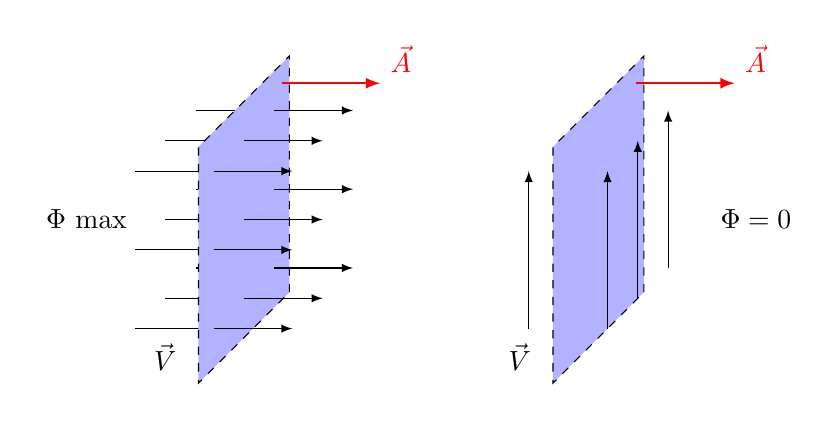
\begin{tikzpicture}[> = latex]

\matrix[column sep = 1 cm]{

 	% Field label
 	
 	\node at (-1, -1.75) {${\vec V}$};
	
	% Field lines (back side)
	
	\foreach \x in {-1, 0, 1}
	\foreach \y in {-1, 0, 1}
	{
		\draw [->] (-1, \x, \y) -- (0, \x, \y);
	}

	% Surface w/area vector
	
	\draw [fill = blue!30, dashed] (0, -1.5, -1.5) -- (0, 1.5, -1.5) -- (0, 1.5, 1.5) -- (0, -1.5, 1.5) -- (0, -1.5, -1.5);
	\draw [->, thick, red] (0, 1.25, -1.25) -- (1.25, 1.25, -1.25) node [above right] {${\vec A}$};
	
	% Field lines (front side)
	
	\foreach \x in {-1, 0, 1}
	\foreach \y in {-1, 0, 1}
	{
		\draw [->] (0, \x, \y) -- (1, \x, \y);
	}
	
	% Flux value
	
	\node at (-2, 0) {$\Phi$ max};
	
&

 	% Field label
 	
 	\node at (-1, -1.75) {${\vec V}$};

	% Field lines (back side)
	
	\foreach \z in {-1, 0, 1}
		\draw [->] (-0.5, -1, \z) -- (-0.5, 1, \z);

	% Surface w/area vector
	
	\draw [fill = blue!30, dashed] (0, -1.5, -1.5) -- (0, 1.5, -1.5) -- (0, 1.5, 1.5) -- (0, -1.5, 1.5) -- (0, -1.5, -1.5);
	\draw [->, thick, red] (0, 1.25, -1.25) -- (1.25, 1.25, -1.25) node [above right] {${\vec A}$};

	% Field lines (front side)
	
	\foreach \z in {-1, 0, 1}
		\draw [->] (0.5, -1, \z) -- (0.5, 1, \z);
	
	% Flux value
	
	\node at (2, 0) {$\Phi = 0$};

\\	
};

\end{tikzpicture}
\end{document}